% Printed 242; principal PDF 249; Google PDF 253.
\par\clearpage
\noindent\makebox[0pt][l]{\fontsize{13}{16}\selectfont 242}\hfill{\small\textbf{BEMERKUNGEN.\quad TRIGONOMETRISCHE PUNKTBESTIMMUNG.}}\hfill\null\par\medskip

{\small
\noindent Punkte geschnitten werden könnten; es genügt, von diesen Punkten andere, die schon festgesetzt sind, einzuschneiden, doch muss die Anzahl derselben wenigstens 3 sein. Hat man 4 geschnitten, so ist eine Controlle da; harmoniren indessen diese 4 nicht, was ebenfalls nicht selten ist, indem eine Verwechselung gar leicht vorfallen kann, so weiss man nicht, wo der Fehler liegt; und deshalb ist es besser, 5 oder noch mehr einzuschneiden. . . . . Überhaupt ist es nicht genug zu empfehlen, jeden Punkt, so oft es nur irgend angeht, einzuschneiden, selbst wenn man nicht Willens ist, die Schnitte nach der Methode der kleinsten Quadrate zu vereinigen, indem man auf diese Art sicher vor Fehlern ist, und ein Punkt, auch wenn er weder Haupt- noch Nebenpunkt ist, sobald er scharf bestimmt ist, häufig dazu dienen kann, die Identität eines andern Punktes zu bestimmen. Hat man nun auch für die Nebenpunkte die Coordinaten berechnet, so geht es an die Bestimmung der übrigen eingeschnittenen Punkte. \textsc{Gauss} führt darüber, nachdem alle\\
\makebox[0pt][r]{.\enspace}Rechnungen abgemacht sind, folgendes Protocoll.
\[
 \overbrace{\text{\textls[120]{Krückeberg}}}^{A}
 \quad\overbrace{-71364{,}939\qquad+45842{,}386}^{B}
\]
\[
\begin{array}{@{}l@{\qquad}r@{\qquad}r@{\qquad}r@{\;}r@{\;}r@{\qquad}r@{}}
 \multicolumn{1}{c}{a}&\multicolumn{1}{c}{b}&\multicolumn{1}{c}{c}&
 \multicolumn{3}{c}{d}&\multicolumn{1}{c@{}}{e}\\
 \text{Süntel}&-70637{,}258&+37481{,}447&94^\circ&58'&27''{,}964&-0{,}885\\
 \text{Klütberg}&-63179{,}059&+41387{,}660&151&26&44{,}009&-1{,}553\\
 \text{Wittekindstein}&-80356{,}285&+71875{,}835&289&3&13{,}703&-0{,}329\\
 \text{Pagenburg}&-75427{,}470&+50454{,}707&311&22&31{,}882&+0{,}448\\
 \hline
 \multicolumn{7}{c@{}}{\text{\textls[120]{Sachsenhagen, Schloss}}\;-96486{,}713\qquad+46075{,}741}\\
 \text{Wittekindstein}&-80356{,}285&+71875{,}835&237&59&11{,}516&\\
 \text{Bergkirchen}&-99061{,}252&+47440{,}144&332&4&3{,}954.&\\
 \hline
\end{array}
\]

\(A\) ist der Ort, dessen Coordinaten bestimmt werden; diese Coordinaten sind sub \(B\) angegeben. \(a\) gibt die Namen der Örter, aus welchen \(A\) bestimmt ist; \(b,c\) ihre Coordinaten; \(d\) das beobachtete Azimuth; \(e\) die Differenz des aus den Coordinaten berechneten und des beobachteten Azimuths, eine Columne, die also wegfällt, sobald wir \textls[120]{nicht mehr} Data haben, als zur Bestimmung des Punkts quaestionis nöthig sind. Geordnet werden die einzelnen in diesem Protocoll aufgenommenen Punkte nicht, doch thut man wohl, etwas Raum überzulassen, um Bemerkungen, die sich später ergeben, und Schnitte, die erst nach dem Berechnen und Eintragen aufgefunden wurden, nachzutragen. Übrigens trägt man die Punkte in dieses Protocoll in der Reihenfolge ein, in welcher sie berechnet sind. In den Tableaux streicht man die Schnitte, die schon zur Berechnung gedient haben, an, um besser übersehen zu können, welche Schnitte noch unerledigt sind.«

Im Nachlass ist noch eine grosse Anzahl solcher Protocolle vorhanden. In dem Arbeitsberichte für 1844 sagt \textsc{Gauss}: »Die Resultate [Coordinaten] sind jedes Jahr nach Verarbeitung der Messungen in Verzeichnisse gebracht, und solcher partiellen Verzeichnisse sind sechzehn vorhanden, welche zusammen etwas über 3000 Bestimmungen enthalten, so jedoch, dass die Anzahl der Punkte selbst etwa um den 7. Theil kleiner sein mag, indem viele Punkte, die in einem spätern Jahre nach dem Hinzukommen neuer Data schärfer oder zuverlässiger bestimmt werden konnten, in mehr als einem Verzeichnisse auftreten. . . . . Zu grösserer Sicherheit und bequemerm Gebrauch habe ich jetzt angefangen, die partiellen Verzeichnisse in Eines zu verschmelzen, welches demnach etwa 2600 Punkte enthalten wird.« (Band IV, S. 413).

In dem Abdruck der aus den Astr. Nachr. entnommenen Abhandlung, Art. 6, sind mehrere Druck- und Rechenfehler berichtigt worden.\hfill\textsc{Krüger.}\par
\begin{center}\rule{4cm}{.4pt}\end{center}
}

% Printed 243; principal PDF 250; Google PDF 254.
\par\clearpage

\thispagestyle{empty}
\vspace*{.23\textheight}
{\centering
{\LARGE AUSGLEICHUNG\par}
\medskip
{\LARGE\bfseries EINFACHER FIGUREN.\par}
}
\vfill
\noindent\hfill31\textsuperscript{*}\hspace*{.15\linewidth}\par
\vspace*{.14\textheight}

% Printed 244; principal PDF 251; Google PDF 255.
\par\clearpage

\null\thispagestyle{empty}

% Printed 245; principal PDF 252; Google PDF 256.
\par\clearpage

\thispagestyle{empty}
\vspace*{3\baselineskip}
{\centering\Large\bfseries NACHLASS UND BRIEFWECHSEL.\par}
\vspace{3\baselineskip}
{\centering
[1.]\par\smallskip
Ausgleichung eines Vierecks.\par}
\begin{flushleft}
\hspace*{1.8em}\(0,1,2,3\) . . . die vier Punkte\\
\hspace*{1.8em}\(01\) . . . . . . . . sowohl Länge als Richtung der Linie \(01\)\\
\hspace*{1.8em}\(C^{01}\), u. s. w. Ausgleichungen, wodurch alles verträglich wird,
\end{flushleft}
\[
 C^{01}=\left[\tfrac12(C^{01}+C^{10})+\tfrac12(C^{01}-C^{10})=\right]S^{01}+D^{01},
\]
\noindent wo
\[
 S^{01}=S^{10},\qquad D^{01}=-D^{10};
\]
{\centering u. s. w.\par}

[Man setze]
\[
 \log\operatorname{hyp}
 \frac{\sin(30-31)\sin(10-12)\sin(20-23)}
      {\sin(32-30)\sin(13-10)\sin(21-20)}
 =\lambda^0
\]
\[
\begin{array}{@{}r@{\;=\;}l@{}}
 12\,.\,13\,.\sin(12-13)&T^0\\
 02\,.\,03\,.\sin(03-02)&T'\\
 03\,.\,13\,.\sin(30-31)&T''\\
 02\,.\,12\,.\sin(21-20)&T'''.
\end{array}
\]

Es bedeuten hier \(T^0,T',T'',T'''\) die vier doppelten Dreiecke; man bemerke, dass allemal zwei Permutationen zugleich gemacht werden müssen: so entsteht \(T'\) aus \(T^0\), wenn \(0\) mit \(1\) und \(2\) mit \(3\) vertauscht wird. Es ist [da \(T^0\) und \(T''\) das entgegengesetzte Vorzeichen von \(T'\) und \(T'''\) haben]
\[
 0=T^0+T'+T''+T'''.
\]
Ebenso entstehen \(\lambda',\lambda'',\lambda'''\) aus \(\lambda^0\).

% Printed 246; principal PDF 253; Google PDF 257.
\par\clearpage
\noindent\makebox[0pt][l]{\fontsize{13}{16}\selectfont 246}\hfill{\small\textbf{NACHLASS.}}\hfill\null\par\medskip

Man hat dann
\[
\resizebox{\linewidth}{!}{\(\begin{aligned}
 {[}0={}&\lambda^0+\frac{\sin(13-12)}{\sin(10-12)\sin(13-10)}C^{10}
 -\operatorname{cotang}(10-12)\,.\,C^{12}
 -\operatorname{cotang}(13-10)\,.\,C^{13}\\
 &+\frac{\sin(21-23)}{\sin(20-23)\sin(21-20)}C^{20}
 -\operatorname{cotang}(21-20)\,.\,C^{21}
 -\operatorname{cotang}(20-23)\,.\,C^{23}\\
 &+\frac{\sin(32-31)}{\sin(30-31)\sin(32-30)}C^{30}
 -\operatorname{cotang}(30-31)\,.\,C^{31}
 -\operatorname{cotang}(32-30)\,.\,C^{32}
\end{aligned}\)}
\]
\noindent oder
\[
\begin{aligned}
 0={}&\lambda^0-\frac{01^2\,.\,T^0}{T''T'''}C^{10}
 -\tfrac12\frac{01^2+12^2-02^2}{T'''}C^{12}
 -\tfrac12\frac{01^2+13^2-03^2}{T''}C^{13}\\
 &-\frac{02^2\,.\,T^0}{T'T'''}C^{20}
 -\tfrac12\frac{02^2+12^2-01^2}{T'''}C^{21}
 -\tfrac12\frac{02^2+23^2-03^2}{T'}C^{23}\\
 &-\frac{03^2\,.\,T^0}{T'T''}C^{30}
 -\tfrac12\frac{03^2+13^2-01^2}{T''}C^{31}
 -\tfrac12\frac{03^2+23^2-02^2}{T'}C^{32}
\end{aligned}
\]
\noindent oder]
\[
\begin{array}{@{}r@{\;}r@{\;}l@{}}
 -T'T''T'''\lambda^0={}&-T^0T'\,.\,01^2\,.\,S^{01}&+T^0T'\,.\,01^2\,.\,D^{01}\\
 &-T^0T''\,.\,02^2\,.\,S^{02}&+T^0T''\,.\,02^2\,.\,D^{02}\\
 &-T^0T'''\,.\,03^2\,.\,S^{03}&+T^0T'''\,.\,03^2\,.\,D^{03}\\
 &-T'T'''\,.\,13^2\,.\,S^{13}&+T'T'''\,.\,(03^2-01^2)D^{13}\\
 &-T'T''\,.\,12^2\,.\,S^{21}&+T'T''\,.\,(01^2-02^2)D^{21}\\
 &-T''T'''\,.\,23^2\,.\,S^{32}&+T''T'''\,.\,(02^2-03^2)D^{32}\\
 =&\Sigma^0&+\qquad\Delta^0.
\end{array}
\]

\(\Sigma',\Sigma'',\Sigma'''\) werden identisch gleich \(\Sigma^0\). \(\lambda^0,\lambda',\lambda'',\lambda'''\) sind den \(T^0,T',T'',T'''\) proportional, wenn die Winkelsummen schon ausgeglichen sind. Hingegen werden \(\Delta',\Delta'',\Delta'''\) numerisch dem \(\Delta^0\) gleich werden müssen, wenn die letztere Ausgleichung conservirt wird. Symmetrisch hat man diesen Werth
\[
\begin{aligned}
 \tfrac14(\Delta^0+\Delta'+\Delta''+\Delta''')=\tfrac14\bigl\{&
 T^0T'D^{01}(12^2+13^2-02^2-03^2)\\
 &+T^0T''D^{02}(12^2+23^2-01^2-03^2)\\
 &+T^0T'''D^{03}(13^2+23^2-01^2-02^2)\\
 &+T'T'''D^{13}(03^2+23^2-01^2-12^2)\\
 &+T'T''D^{21}(01^2+13^2-02^2-23^2)\\
 &+T''T'''D^{32}(02^2+12^2-03^2-13^2)\bigr\}.
\end{aligned}
\]

Jedes \(\Delta=H^{01}D^{01}+H^{02}D^{02}+\cdots\) gesetzt, wird in die Form gebracht, wo die Summe der Quadrate der Coefficienten ein Minimum wird, indem man

% Printed 247; principal PDF 254; Google PDF 258.
\par\clearpage
\noindent\null\hfill{\small\textbf{AUSGLEICHUNG EINFACHER FIGUREN.}}\hfill\makebox[0pt][r]{\fontsize{13}{16}\selectfont 247}\par\medskip

\noindent schreibt
\[
\begin{array}{@{}l@{\;}l@{\;}l@{}}
 \text{anstatt}&
 H^{01}\,.\,.\,.\,.\,.\,.\,.\,.&
 \tfrac14(2H^{01}-H^{20}-H^{30}+H^{21}+H^{31})\\
 \text{\quad»}&
 H^{02}\,.\,.\,.\,.\,.\,.\,.\,.&
 \tfrac14(2H^{02}-H^{10}-H^{30}+H^{12}+H^{32})\\
 \multicolumn{3}{c@{}}{\text{u. s. w.,}}
\end{array}
\]
\noindent wo \(H^{\alpha\beta}=-H^{\beta\alpha}\).

[Addirt man nemlich zu dem Ausdrucke für \(\Delta^0\) die 3 Winkelgleichungen, welche \(T',T'',T'''\) entsprechen und die bereits ausgeglichen sein sollen, nachdem man sie mit den Factoren \(\tfrac12\mu_1,\tfrac12\mu_2,\tfrac12\mu_3\) multiplicirt hat, so wird \(\Delta^0\) nicht geändert. (Die Constante \(\lambda^0\) muss natürlich jetzt auch mit den Werthen berechnet sein, die die Ausgleichung der Winkelgleichungen ergeben hat). Es ist also auch, da hienach die Winkelgleichungen lauten
\[
 \resizebox{\linewidth}{!}{\(0=-C^{02}+C^{03}-C^{23}+C^{20}-C^{30}+C^{32}
 =2(-D^{02}+D^{03}+D^{32}),\ \text{u. s. w.:}\)}
\]
\[
\begin{aligned}
 \Delta^0={}&H^{01}D^{01}+H^{02}D^{02}+H^{03}D^{03}
             +H^{13}D^{13}+H^{21}D^{21}+H^{32}D^{32}\\
 &+\mu_1(-D^{02}+D^{03}+D^{32})+\mu_2(-D^{01}+D^{03}-D^{13})\\
 &\hspace{3.3em}+\mu_3(-D^{01}+D^{02}+D^{21}).
\end{aligned}
\]

Bestimmt man nun \(\mu_1,\mu_2,\mu_3\) in der Weise, dass die Summe der Quadrate der Coefficienten von \(D^{01},D^{02}\), u. s. w. ein Minimum wird, so wird
\[
\begin{array}{@{}r@{\;}r@{\;}r@{\;=\;}l@{}}
 3\mu_1&+\mu_2&-\mu_3&H^{02}-H^{03}-H^{32}\\
 \mu_1&+3\mu_2&+\mu_3&H^{01}-H^{03}+H^{13}\\
 -\mu_1&+\mu_2&+3\mu_3&H^{01}-H^{02}-H^{21},
\end{array}
\]
\noindent also
\[
\begin{array}{@{}r@{\;=\;}l@{}}
 \mu_1&\tfrac14(H^{02}-H^{03}-H^{13}-H^{21}-2H^{32})\\
 \mu_2&\tfrac14(H^{01}-H^{03}+2H^{13}+H^{21}+H^{32})\\
 \mu_3&\tfrac14(H^{01}-H^{02}-H^{13}-2H^{21}-H^{32});
\end{array}
\]
\noindent damit ergibt sich:
\[
\begin{array}{@{}r@{\;}r@{\;}r@{\;}r@{\;}r@{\;}r@{\;}r@{\;}l@{}}
 4\Delta^0=&(\,2H^{01}&+H^{02}&+H^{03}&-H^{13}&+H^{21}&\ast&\,)D^{01}\\
 +(&H^{01}&+2H^{02}&+H^{03}&\ast&-H^{21}&+H^{32}&)D^{02}\\
 +(&H^{01}&+H^{02}&+2H^{03}&+H^{13}&\ast&-H^{32}&)D^{03}\\
 +(&-H^{01}&\ast&+H^{03}&+2H^{13}&-H^{21}&-H^{32}&)D^{13}\\
 +(&H^{01}&-H^{02}&\ast&-H^{13}&+2H^{21}&-H^{32}&)D^{21}\\
 +(&\ast&+H^{02}&-H^{03}&-H^{13}&-H^{21}&+2H^{32}&)D^{32}.
\end{array}
\]

Dieser Ausdruck lässt sich in den folgenden umwandeln:

% Printed 248; principal PDF 255; Google PDF 259.
\par\clearpage
\noindent\makebox[0pt][l]{\fontsize{13}{16}\selectfont 248}\hfill{\small\textbf{NACHLASS UND BRIEFWECHSEL.}}\hfill\null\par\medskip

\[
\resizebox{\linewidth}{!}{\(\begin{array}{@{}r@{}r@{\;}r@{\;}r@{\;}r@{\;}r@{\;}r@{\;}r@{}l@{}}
 4\Delta^0=&\{&\ast&+02^2\,.\,T^0T''&+03^2\,.\,T^0T'''&-12^2\,.\,T'T''&-13^2\,.\,T'T'''&\ast&\}D^{01}\\
 +&\{&+01^2\,.\,T^0T'&\ast&+03^2\,.\,T^0T'''&-12^2\,.\,T'T''&\ast&-23^2\,.\,T''T'''&\}D^{02}\\
 +&\{&+01^2\,.\,T^0T'&+02^2\,.\,T^0T''&\ast&\ast&-13^2\,.\,T'T'''&-23^2\,.\,T''T'''&\}D^{03}\\
 +&\{&-01^2\,.\,T^0T'&+02^2\,.\,T^0T''&\ast&\ast&-13^2\,.\,T'T'''&+23^2\,.\,T''T'''&\}D^{21}\\
 +&\{&+01^2\,.\,T^0T'&\ast&-03^2\,.\,T^0T'''&+12^2\,.\,T'T''&\ast&-23^2\,.\,T''T'''&\}D^{13}\\
 +&\{&\ast&-02^2\,.\,T^0T''&+03^2\,.\,T^0T'''&-12^2\,.\,T'T''&+13^2\,.\,T'T'''&\ast&\}D^{32}.
\end{array}\)}
\]

Zu dem gleichen Werthe gelangt man, wenn man die entsprechenden Entwickelungen für \(\Delta',\Delta'',\Delta'''\) macht; man erkennt dies auch daraus, dass für die Vertauschungen, die \(\Delta^0\) in \(\Delta',\Delta'',\Delta'''\) überführen, die rechten Seiten der obigen und der vorhergehenden Gleichung ungeändert bleiben, wenn man berücksichtigt, dass \(D^{ik}=-D^{ki}\) ist. \(\Delta^0\) geht z. B. in \(\Delta'\) über, wenn man \(0\) mit \(1\), \(2\) mit \(3\) und ebenso \({}^0\) mit \({}'\) und \({}''\) mit \({}'''\) vertauscht. Es ist mithin, vorausgesetzt, dass die Winkelgleichungen des Dreiecks vor Aufstellung der Seitengleichungen bereits ausgeglichen waren:
\[
 T'T''T'''\lambda^0=T^0T''T'''\lambda'=T^0T'T'''\lambda''=T^0T'T''\lambda'''
\]
\noindent oder
\[
 \frac{\lambda^0}{T^0}=\frac{\lambda'}{T'}=\frac{\lambda''}{T''}=\frac{\lambda'''}{T'''}.\biggr]
\]

\medskip
{\centering
[2.]\par\smallskip
Gleichung zwischen den Seiten und Diagonalen eines Vierecks.\par}
Zwischen den Seiten und \(T',T'',T'''\) gibt es die Gleichungen
\[
\begin{aligned}
 0={}&2\,.\,01^2\,.\,T'+(01^2+02^2-12^2)T''+(01^2+03^2-13^2)T'''\\
 0={}&(01^2+02^2-12^2)T'+2\,.\,02^2\,.\,T''+(02^2+03^2-23^2)T'''\\
 0={}&(01^2+03^2-13^2)T'+(02^2+03^2-23^2)T''+2\,.\,03^2\,.\,T'''.
\end{aligned}
\]
Schreibt man dafür
\[
\begin{aligned}
 0&=AT'+cT''+bT'''\\
 0&=cT'+BT''+aT'''\\
 0&=bT'+aT''+CT''',
\end{aligned}
\]
\noindent so wird
\[
 ABC+2abc=aaA+bbB+ccC,
\]
\noindent welches die zwischen den sechs Seiten stattfindende Bedingungsgleichung ist.

% Printed 249; principal PDF 256; Google PDF 260.
\par\clearpage
\noindent\null\hfill{\small\textbf{AUSGLEICHUNG EINFACHER FIGUREN.}}\hfill\makebox[0pt][r]{\fontsize{13}{16}\selectfont 249}\par\medskip

Entwickelt gibt dies:
\[
\begin{aligned}
 &01^2\,.\,23^2\{02^2+03^2+12^2+13^2\}-01^4\,.\,23^2-01^2\,.\,23^4\\
 +{}&02^2\,.\,13^2\{01^2+03^2+12^2+23^2\}-02^4\,.\,13^2-02^2\,.\,13^4\\
 +{}&03^2\,.\,12^2\{01^2+02^2+13^2+23^2\}-03^4\,.\,12^2-03^2\,.\,12^4\\
 ={}&01^2\,.\,02^2\,.\,12^2+01^2\,.\,03^2\,.\,13^2+02^2\,.\,03^2\,.\,23^2+12^2\,.\,13^2\,.\,23^2.
\end{aligned}
\]

\medskip
{\centering
[3.]\par\smallskip
[Über die Wahl der Bedingungsgleichung aus den Seitenverhältnissen.]\par\smallskip
\textsc{Gauss} an \textsc{Gerling}. \quad Göttingen, 11. Februar 1824.\par}

. . . . . . \textit{Zur} Prüfung des Vierecks haben Sie eine Bedingungsgleichung mit acht Factoren; es ist aber nur eine mit \textls[120]{sechs} nöthig, die auf 4 verschiedene Arten eingekleidet werden kann:

\begin{center}
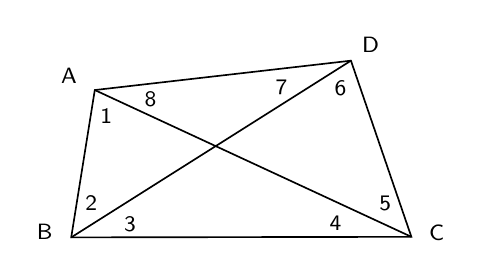
\begin{tikzpicture}[x=.72cm,y=.72cm,line width=.6pt,font=\footnotesize\sffamily]
 \coordinate (A) at (.416,2.599);
 \coordinate (B) at (0,0);
 \coordinate (C) at (6,.01);
 \coordinate (D) at (4.934,3.117);
 \draw (A)--(B)--(C)--(D)--cycle;
 \draw (A)--(C) (B)--(D);
 \node at (-.041,2.843) {A};
 \node at (-.467,.091) {B};
 \node at (6.447,.081) {C};
 \node at (5.279,3.401) {D};
 \node at (.619,2.132) {1};
 \node at (.355,.609) {2};
 \node at (1.035,.233) {3};
 \node at (4.66,.253) {4};
 \node at (5.54,.61) {5};
 \node at (4.75,2.63) {6};
 \node at (3.71,2.64) {7};
 \node at (1.40,2.44) {8};
\end{tikzpicture}
\end{center}
\[
\left.\begin{array}{@{}l@{\;=\;}l@{}}
 \sin1\,.\sin3\,.\sin(6+7)&\sin(2+3)\,.\sin6\,.\sin8\\
 \sin3\,.\sin5\,.\sin(8+1)&\sin(4+5)\,.\sin8\,.\sin2\\
 \sin5\,.\sin7\,.\sin(2+3)&\sin(6+7)\,.\sin2\,.\sin4\\
 \sin7\,.\sin1\,.\sin(4+5)&\sin(8+1)\,.\sin4\,.\sin6.
\end{array}\right\}\quad\text{\tikz[baseline=-.55ex,x=1mm,y=1mm,line width=.4pt]{\draw (0,1.2)--(-1.25,-.6)--(1.25,-.6)--cycle;\draw (0,-1.2)--(-1.25,.6)--(1.25,.6)--cycle;}}
\]

Am vortheilhaftesten ist es, die \(1^{\mathrm{te}},2^{\mathrm{te}},3^{\mathrm{te}}\) oder \(4^{\mathrm{te}}\) Form anzuwenden, je nachdem das Dreieck \(ABD,ABC,BCD,ACD\) am grössten ist.

Es ist mir nicht recht deutlich, wie Sie sich die Art, \raisebox{.8ex}{.}\,eine gemessene Diagonalrichtung zu benutzen, gedacht haben\textsuperscript{[*)]}. Es folgt ja daraus, dass, wenn sechs Grössen \(A,B,C,D,E,F\) gemessen wären, zwischen deren Correctionen eine Bedingungsgleichung
\[
 \partial A-\partial B+\partial C-\partial D+\partial E-\partial F=\text{Quant. data}
\]

\par\noindent\rule{4cm}{.4pt}\par
{\footnotesize\noindent\hspace*{\parindent}[*) \textsc{Gerling} glaubte, noch zwei Winkelgleichungen, je mit dem Absolutgliede Null, ansetzen zu müssen, wenn in einem Viereck die eine Diagonale nur einseitig beobachtet ist.]\par}
\noindent{\small IX.}\hfill{\small 32}\hspace*{.12\linewidth}\par

% Printed 250; principal PDF 257; Google PDF 261.
\par\clearpage
\noindent\makebox[0pt][l]{\fontsize{13}{16}\selectfont 250}\hfill{\small\textbf{BRIEFWECHSEL.}}\hfill\null\par\medskip

\noindent stattfinden würde, nunmehro, weil die sechste, \(F\), \textls[120]{nicht} gemessen ist, die Bedingungsgleichung
\[
 \partial A-\partial B+\partial C-\partial D+\partial E=0
\]
\noindent stattfinden müsse. Vielmehr ist eine solche Bedingungsgleichung durchaus unzulässig, und die beiden, die Sie anführen, addirt, würden sogar etwas in directem Widerspruch mit dem Übrigen stehendes geben.

Alle Diagonal-Einschnitte können lediglich durch \textls[120]{diejenigen} Bedingungsgleichungen mit benutzt werden, die solche Gleichungen, wie die oben mit \mbox{\tikz[baseline=-.55ex,x=1mm,y=1mm,line width=.4pt]{\draw (0,1.2)--(-1.25,-.6)--(1.25,-.6)--cycle;\draw (0,-1.2)--(-1.25,.6)--(1.25,.6)--cycle;}} bezeichneten, an die Hand geben. Es macht dabei gar keinen Unterschied, ob der Einschnitt auch reciprok stattgefunden hat oder nicht; es kommt bloss im ersten Fall noch diejenige Bedingungsgleichung hinzu, die aus der Winkelsumme des Einen Dreiecks entsteht (die aus dem andern [Dreiecke] ist dann implicite schon in den übrigen enthalten), welche im andern [Falle] wegfällt.

Übrigens wiederhole ich, dass alles viel einfacher in derjenigen Behandlungsmethode ausfällt, die ich vorzugsweise für meine Messungen gewählt habe. Übrigens kommt in meinem eigenen Hauptdreieckssystem gar keine solche Diagonale vor, die nicht auch reciprok gemessen wäre; die wenigen der Art, die an den Grenzen vorkommen, als Hohehagen—Meisner, etc., verschiedene neue Dreieckspunkte, Syk und Hohenhorn, habe ich gar nicht ins System aufgenommen, sondern bisher alle Ausgleichung nur auf die vollständige Messung gegründet, die andern Punkte aber gleichsam als Nebenpunkte betrachtet, in Beziehung auf welche die Lage meiner Hauptpunkte als absolut genau betrachtet ist. . . . . . .

\bigskip
{\centering
\textsc{Gauss} an \textsc{Gerling}. \quad Göttingen, 19. Januar 1840.\par}
\medskip

. . . . . . Das Durchlesen Ihrer schönen Schrift über Ihre \(\Delta\Delta\) hat mich veranlasst, mich etwas wieder in die Sache hineinzudenken, und einige Bemerkungen werden vermuthlich für Sie nicht ohne Interesse sein. Obgleich ich Ihnen vorausgesagt hatte, dass, bei der Zickzack-Behandlung der Bedingungsgleichungen nach zwei Gruppen, Sie nur eine langsame Convergenz haben würden, so war ich doch etwas verwundert, dass Sie nach einem Ihrer Briefe

% Printed 251; principal PDF 258; Google PDF 262.
\par\clearpage
\noindent\null\hfill{\small\textbf{AUSGLEICHUNG EINFACHER FIGUREN.}}\hfill\makebox[0pt][r]{\fontsize{13}{16}\selectfont 251}\par\medskip

\noindent 15-mal alles durchgemacht haben (nach dem Buche 13-mal; ich weiss nicht, wie diese Discordanz zu erklären ist). Bei meinem eigenen Gradmessungssystem hatte ich gegen 50 Bedingungsgleichungen der zweiten und 12 von der dritten Art; aber hier war die Convergenz sehr schnell, so dass schon die dritte [Rechnung] in der \(\frac{1}{1000}''\) stehende Resultate gab. Aber freilich wäre dies nicht möglich gewesen ohne einen besondern Kunstgriff, den Sie, wie mir scheint, \textls[120]{nicht} benutzt haben. Ob ich ihn Ihnen vor 15 Jahren angezeigt habe (in einem Ihrer Briefe beziehen Sie sich auf damals gemachte Mittheilungen), weiss ich nicht, ich bin aber auch ungewiss, ob ich damals ihn schon selbst ausgeübt hatte; meine grossen Ausgleichungsrechnungen sind, glaube ich, Anfang 1826 gemacht, ich habe aber nirgends eine Zeit notirt. Ich will versuchen, Ihnen eine Idee davon zu geben, obwohl eine ausführliche Entwickelung eine ziemlich starke Abhandlung geben könnte.

Ich nehme also an, die Ausgleichung auf die von den Winkelsummen abhängigen Bedingungsgleichungen sei schon einmal gemacht, und man wolle nun auf die Bedingungsgleichungen durch Seitenverhältnisse übergehen. Ich betrachte Kürze halber bloss ein Vierpunktsystem \(0\,.\,1\,.\,2\,.\,3\). Ist von den vier \(\Delta\Delta\) \(123\) das grösste, so benutzen Sie die Formel \(\frac{01}{02}\,.\,\frac{02}{03}\,.\,\frac{03}{01}=1\) (hier sind \(01\), u. s. w. Seiten: von jetzt an bezeichne ich aber mit \(01\) den \textls[120]{Winkel}, welchen diese Seite mit der Zerolinie in \(0\) macht). Jene Gleichung gibt Ihnen \textls[120]{unmittelbar} eine Bedingungsgleichung zwischen \(9\) Correctionen; es erscheinen nemlich nicht mit: \(\mathrm{d}01,\mathrm{d}02,\mathrm{d}03\). Hätten Sie die Formel \(\frac{10}{12}\,.\,\frac{12}{13}\,.\,\frac{13}{10}=1\) gebraucht, so hätten Sie eine Bedingungsgleichung zwischen \textls[120]{9 andern} Correctionen erhalten; es würden nemlich \(\mathrm{d}10,\mathrm{d}12,\mathrm{d}13\) gefehlt haben. Diese beiden Bedingungsgleichungen sind also nicht identisch, aber man kann die eine aus der andern ableiten, wenn man diejenigen Bedingungsgleichungen der zweiten Art, welche dem Viereck angehören, mit zuzieht. Hier tritt nun ein Fall ein, der oft vorkommt, und wo ein nicht genug zu preisender Rath seine Anwendung findet. Nemlich wenn bei einer Untersuchung die Bestandtheile symmetrisch vorliegen, und man kann auf mehr als Eine Weise zum Ziel kommen, wovon die eine so gut scheint wie die andere, und wo man also sich im Fall von Buridans Esel befindet, so soll man \textls[120]{keinen dieser Wege wählen}, sondern einen andern suchen, wo allen Bestandtheilen gleiches Recht wiederfährt. Darüber lassen sich freilich keine allgemeinen Regeln geben,
\par\smallskip
\noindent\hfill{\small 32\textsuperscript{*}}\hspace*{.12\linewidth}\par
